\documentclass{standalone}
\usepackage{tikz}
\usepackage{ctex,siunitx}
\setCJKmainfont{Noto Serif CJK SC}
\usepackage{tkz-euclide}
\usepackage{amsmath}
\usetikzlibrary{patterns, calc}
\usetikzlibrary {decorations.pathmorphing, decorations.pathreplacing, decorations.shapes,}

\begin{document}
\small
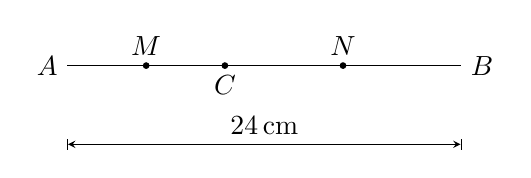
\begin{tikzpicture}[>=stealth,scale=1]
  \tkzSetUpPoint[fill=black]
  % \useasboundingbox(-1,-0.75)rectangle(3.7,1.4);
  \draw(0,0)node[left]{$A$}--(5,0)node[right]{$B$};
  \tkzDefPoints{1/0/M, 2/0/C, 3.5/0/N}
  \tkzDrawPoints(M,C,N)
  \tkzLabelPoints[above](M,N)
  \tkzLabelPoint[below](C){$C$}
  \draw[|<->|, very thin](0,-1)--(5,-1)node[midway,above]{\qty{24}{cm}};
\end{tikzpicture}
\end{document}